\cleardoublepage
\section{Umsetzung} \thispagestyle{nomarkstyle}
Hier werden konkret alle Aspekte der Umsetzung der in \cref{specification} bereits beschriebenen Spezifikation behandelt. %TODO umschreiben
 
\subsection{Initiales Aufsetzen der Anwendung}
Bevor die Entwicklung starten kann müssen die grundlegende Bausteine der Anwendung angelegt, konfiguriert und verbunden werden. 

\subsubsection{Spring Boot Anwendung}\label{spring-boot-init}
Spring stellt eine Weboberfläche zur Verfügung, in der ein komplettes Spring Boot Projekt inklusive Abhängigkeiten einfach generiert werden kann. Die Oberfläche (namens Spring Initializr) erlaubt es Maven oder Gradle als Build-Management-Tool zu verwenden. In diesem Projekt fiel die Entscheidung für Maven, aufgrund der bereits vorhandenen Erfahrung mit dem Tool. 

\begin{figure}[th!]
	\centering
	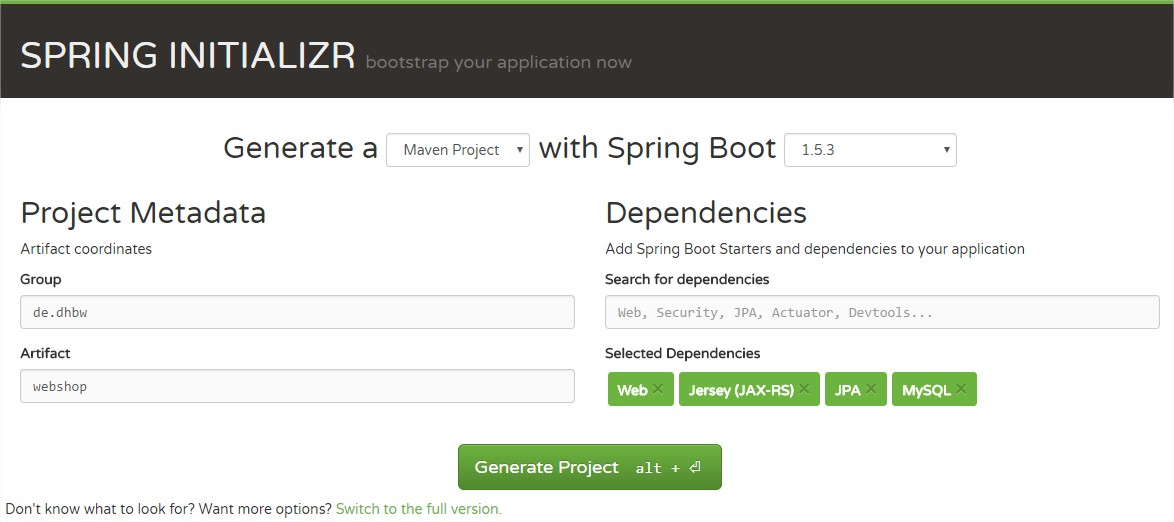
\includegraphics[width=\linewidth]{bilder/kap7/Spring-Initializr}
	\caption{Spring Inititalizr Weboberfläche}
	\label{fig:spring-initializr}
\end{figure}

\cref{fig:spring-initializr} zeigt die gewählte Konfiguration für das Grundprojekt. Links sind die Metadaten für das Deployment definiert und rechts die Abhängigkeiten. Diese sind initial:

\begin{itemize}
	\item \textit{Spring Web}. Benötigt um eine Webanwendung mit eingebetteten Tomcat-Server zu implementieren.
	\item \textit{Jersey}. Hierbei handelt es sich um die Referenzimplementierung von JAX-RS. JAX-RS ermöglicht es, anhand von Annotationen, herkömmliche Java-Klassen per REST verfügbar zu machen. Für die Darstellung dieser Ressourcen verwendet JAX-RS standardmäßig die Implementierung von \acs{JAXB} (Java Architecture for XML Binding). Der Vorteil daran ist, dass die Klassen mit der Annotation \texttt{@XmlRootElement} automatisch bei einem REST Aufruf in die entsprechende XML oder \acs{JSON} Darstellung umgewandelt werden. Die Unterstützung des JSON Formates ist dadurch gewährleistet, dass JAXB die Jackson Bibliotheken benutzt. Die Jackson Bibliothek bietet einen mächtigen Parser für die Konvertierung von Java-Objekten in JSON-Strings\footcite[Vgl.][]{Oracle2015}.
	\item \textit{Spring Data JPA}. Stellt die Zugriffstechnologie der Java Persistence API (\acs{JPA}) zur Verfügung. Mit dieser Abhängigkeit können Datenzugriffsobjekte angelegt werden (sogenannte \acs{DAO}s, Data Access Objects), die alle notwendige Datenbankoperationen implementieren\footcite[Vgl.][]{Webb2017}. 
	\item \textit{Spring MySQL JDBC Driver}. Damit kann die Spring Boot Anwendung automatisch eine Verbindung zur MySQL-Datenbank herstellen\footcite[Vgl.][]{Webb2017}. Alle weitere Konfigurationen für diese Verbindung werden später in dieser Arbeit beschrieben.
\end{itemize}

Die Ordnerstruktur des generierten Projekts kann der \cref{fig:init-project} entnommen werden. Es handelt sich hierbei um die übliche Struktur einer Java-Anwendung, mit einem \texttt{main} und einem \texttt{test} Verzeichnis. Initial sind im \texttt{main} Verzeichnis nur zwei Dateien: die \texttt{WebshopApplication} Klasse und die \texttt{application.properties}. Erstere enthält die Java \texttt{main}-Methode, welche die Anwendung lauffähig macht. Dort werden auch automatisch alle notwendige Konfigurationen für Spring Boot gesetzt. Die \texttt{application.properties} Datei ist zu diesem Zeitpunkt noch leer, aber sie wird später benutzt um unterschiedliche Aspekte der Anwendung (wie zum Beispiel Server-Port oder Verbindungsdaten zur Datenbank) auf einer einfachen Art und Weise einzustellen.

Eine weitere wichtige Datei ist die \texttt{pom.xml} im Stammverzeichnis. Das Project Object Model oder \acs{POM} ist die grundlegende Arbeitseinheit von Maven. Die XML-Datei enthält Information über das Projekt, sowie Konfigurationsdetails welche von Maven verwendet werden um das Projekt zu bauen. Einige dieser Konfigurationen sind Projekt-Abhängigkeiten, Plugins, Build-Profile usw.\footcite[Vgl.][]{Foundation2017}

\begin{figure}[th!]
	\centering
	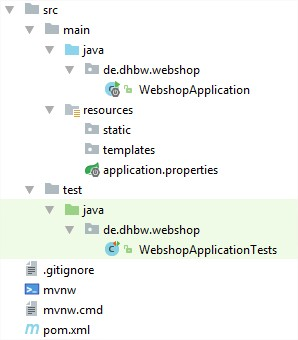
\includegraphics[width=0.5\linewidth]{bilder/kap7/init-project}
	\caption{Ordnerstruktur des generierten Projekts}
	\label{fig:init-project}
\end{figure}

\subsubsection{Angular 2 Anwendung}
Auch hier wird ein Tool eingesetzt, um eine Basisanwendung zu generieren. Hierbei handelt es sich um die Angular CLI, ein Tool für die Initialisierung, Entwicklung und Wartung von Angular Anwendungen\footcite[Vgl.][]{Arora2017}. 

Angular CLI ist ein Open Source Projekt und wird anhand des Node Package Managers (\acs{NPM}) installiert. Daraufhin stehen zahlreiche nützliche Befehle für die Kommandozeile zur Verfügung. Für das Generieren einer Angular-Anwendung wird \texttt{ng init} ausgeführt. Der Befehl erstellt alle notwendige Ressourcen, sowie die komplette Konfiguration dazu. Die statische Inhalte werden mit \texttt{ng build} gebaut. 

Damit Spring Boot diese Inhalte verwenden kann müssen sie jedoch im  \texttt{resources/static} Verzeichnis (siehe \cref{fig:init-project}) liegen. Das kann durch einer Anpassung an der \texttt{angular-cli.json} Datei erreicht werden (Zeile 4 von \cref{lst:angular-cli}). Des weiteren enthält diese Datei auch weitere wichtige Konfigurationen, wie der Ablageort von anderen Ressourcen wie Bilder oder benötigte Stylesheets. An dieser Stelle werden demnach die \acs{CSS}-Dateien für das Bootstrap Framework referenziert, sowie eine eigene Stylesheet für weitere Anpassungen. Mehr zu Bootstrap und zu den Designentscheidungen wird später in dieser Arbeit behandelt.
\\
\lstinputlisting[language=json,firstline=7,lastline=10,caption=Auszug der Datei angular-cli.json,label=lst:angular-cli]{listings/angular-cli.json}

\subsection{Backend-Klassen}
Wie bereits in \cref{outline_datamodel} beschrieben, gibt es für jede Entität in der Datenbank eine Klasse, die sie repräsentiert.
Um einzelne Datensätze aus der Datenbank zur Laufzeit in der Anwendung verwenden zu können, gibt es sogenannte \acs{DAO}-Klassen.
Diese gewährleisten den Zugriff auf die Datenbank und bieten außerdem Funktionen an, um bestimmte Datensätze über Abfragekriterien zu finden.
Von den \acs{DAO}-Klassen gelieferte Datensätze können als Instanzen der repräsentierenden Klasse weiterverwendet werden.
Für die Realisierung dieser Zugriffs-Klassen wurden Spring Data \acs{JPA} Repositories verwendet, die neben den grundlegenden \acs{CRUD}-Operationen eine Vielzahl an möglichen Abfragen ermöglichen.
\\
\lstinputlisting[language=Java,breaklines=true, firstline=15,caption=CategoryDao.java,label=lst:CategoryDao]{listings/CategoryDao.java}

\cref{lst:CategoryDao} zeigt eine solche \acs{DAO}-Klasse.
Zugriffs-Funktionen zu definieren kann auf unterschiedliche Art und Weise passieren. Zum einen ermöglichen diese Repositories es, Suchkriterien über den Namen der jeweiligen Funktion zu definieren.
So kann beispielsweise über eine Funktion \textit{findByName(String name)} der Datensatz mit dem der Funktion übergebenen Namen gefunden werden, wenn die Tabelle eine Spalte mit der Bezeichnung \enquote{Name} enthält. Die Zuordnung auf die entsprechende Spalte in der Tabelle und die Suchfunktionalität müssen dabei nicht vom Entwickler implementiert werden.
Neben diesen semi-automatischen Funktionen können aber auch eigene Methoden definiert werden. Dafür kann über eine Annotation (@Query)eine \acs{SQL}-Query für die Abfrage an die Datenbank definiert werden.

\subsection{Objektrelationale Abbildung (\acs{ORM}) mit Hibernate}
Für die Zuordnung der Backend-Klassen zu der entsprechenden Tabelle in der Datenbank mit Hibernate stehen dem Entwickler eine Vielzahl von Annotationen zur Verfügung, von denen einige hier kurz beschrieben werden sollen.
Die Hibernate Annotation um eine Klasse als Entität zu markieren ist denkbar einfach. Sie wird direkt über der Klassendefinition mit \textit{@Entity} gesetzt.
Darüber hinaus können auch der Tabellen-Name sowie die Namen der einzelnen Tabellenspalten über der Definition der Klasse beziehungsweise des Attributs gesetzt werden. Das ist allerdings nur für den Fall nötig, wenn diese Namen explizit vergeben werden sollen.
Wenn man die Zuordnung für eine bereits bestehende Datenbank machen möchte, sind diese expliziten Namen sehr hilfreich.
Ist eine entsprechende Tabelle beim Start der Anwendung nicht vorhanden, wird diese von Hibernate erzeugt.

Eine weitere wichtige Annotation betrifft die Primärschlüssel der Tabelle, die jeden Datensatz eindeutig identifizieren können. Mit \textit{@Id} kann dieses Attribut gekennzeichnet werden.
Empfehlenswert ist dabei die Verwendung eines künstlichen Schlüssels als Zahlenwert, der für jeden Eintrag hochgezählt wird.
Auch dafür bietet Hibernate eine komfortable Lösung, indem über \textit{@GeneratedValue} ein solcher generierter Wert definiert wird.
In Kombination mit einer automatischen Inkrementierung, die MySQL für numerische Werte bietet, kann also automatisch ein eindeutiger Zahlenwert für jeden neuen Eintrag in der Tabelle gesetzt werden.

Für die Beziehungen zu anderen Entitäten können entsprechend der Kardinalität folgende Annotationen verwendet werden:
\begin{itemize}
\item{@OneToOne}
\item{@OneToMany}
\item{@ManyToOne}
\item{@ManyToMany}
\end{itemize}

Über Parameter dieser Annotationen können neben der Ziel-Entität weitere Einstellungen (beispielsweise zum Cascading) gemacht werden, auf die hier nicht näher eingegangen werden soll.

\subsubsection{Vererbung von Klassen}
Eine Vererbungshierarchie von Klassen kann mit verschiedenen Strategien in der Datenbank abgebildet werden.
Hibernate bietet dafür vier grundlegende Varianten an \footcite[Vgl.][]{Mihalcea2017}:
\paragraph{Mapped Superclass}$\;$ \\
In dieser einfachsten Form der Abbildung einer Vererbung wird für jede konkrete Ausprägung der vererbenden Klasse eine eigene Tabelle angelegt, die neben ihren eigenen auch alle Spalten der Eltern-Klasse enthält.
Die Vererbungshierarchie wird damit nicht explizit im Datenmodell ersichtlich.
\paragraph{Single table}$\;$ \\
Dabei werden alle erbenden Klassen in einer einzigen Tabelle in der Datenbank abgebildet. Dadurch enthält die Tabelle viele Spalten, da alle Attribute jeder Sub-Klasse enthalten sind.
Für einzelne Datensätze einer bestimmten erbenden Klasse werden nicht benötigte Spalten mit \enquote{null}-Werten belegt.
Um zu unterscheiden welche Datensätze zu welcher Sub-Klasse gehören wird außerdem eine sogenannte \enquote{Discriminator Column} definiert.
Dieser Ansatz ist sehr performant, da für Abfragen immer nur eine Tabelle verwendet werden muss.
\paragraph{Table-per-subclass}$\;$ \\
Hier wird für die vererbende und jede erbende Klasse eine eigene Tabelle in der Datenbank erzeugt. Letzere enthalten dabei nur die Attribute, die sie zusätzlich zu den der Eltern-Klasse haben. Die Zuordnung zur Eltern-Klasse wird über JOINS hergestellt, was die Performanz bei häufigen Abfragen negativ beeinflussen kann.
\paragraph{Table-per-concrete-class}$\;$ \\
In dieser letzten Variante wird wie bei Table-per-subclass für alle Entitäten eine Tabelle erzeugt. Diese enthalten jedoch jeweils alle eigenen und die Attribute der Eltern-Klasse.
Die Zuordnung wird über UNION-Operationen hergestellt, was ebenfalls zu Performance-Verlusten bei großen Klassen-Hierarchien führen kann.

Innerhalb des Webshops wurde für die Hierarchie bei Artikeln die \enquote{Single Table}-Strategie gewählt.
\cref{lst:inheritanceMapping} zeigt die Klassen-Definitionen mit den Annotationen für das \acs{ORM}.
\\
\lstinputlisting[language=Java, breaklines=true, caption=Vererbungshierarchie, label=lst:inheritanceMapping]{listings/Inheritance.java}

\subsection{REST-Schnittstellen}

%TODO Aufbau der Rest-Interfaces + Implementierungen, evtl. Klassendiagramme. 

In \cref{spring-boot-init} wurde bereits erwähnt, dass für das Erstellen von REST-Services innerhalb der Spring Boot Anwendung Jersey benutzt wird. 

\subsection{Frontend}
%TODO Erstellte Module in Angular 2 (was sind Module? -> Erklären), Struktur von Komponenten, Hauptkomponenten der Module, Services, Routing

\subsubsection{Module}

\subsubsection{Komponenten}

\subsubsection{Services}

\subsubsection{Routing}

\subsubsection{Styling}
